\chapter[Implementación]{
  \label{chp:implementacion}
  IMPLEMENTACIÓN
}
\thispagestyle{numberingStyle}
\pagestyle{numberingStyle}



\section{Estructura de la aplicación}
\subsection{Estructura proyecto Java}
Para la implementación del servicio del modelo y del servidor de aplicación web, se ha elaborado un proyecto Maven con los siguientes módulos:
\\
\\

\begin{figure}[H]
\centering
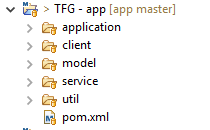
\includegraphics[
   keepaspectratio=true
]{./06_Implementacion/img/estructuraglobaljava.png}
\caption{Estructura proyecto Java}
\end{figure}


\begin{itemize}
	\item \textbf{TFG - app: } Es el proyecto Maven de la aplicación Java. Está formado por diferentes módulos que forman la aplicación:
	\begin{itemize}
		\item \textbf{Application: } Es un módulo donde se encuentran los dos servicios web del sistema: el servicio REST y la aplicación web
		\item \textbf{Client: } Es un módulo donde se implementa el cliente que consuma los servicios REST, necesario para la aplicación web
		\item \textbf{Model: } Donde reside la persistencia y la lógica de negocio de la aplicación.
		\item \textbf{Service : } Es el módulo que define e implementa los recursos REST ofrecidos.
		\item \textbf{Util : } Módulo de utilidad. Aporta clases y funciones comunes a los demás módulos.
		\item \textbf{pom.xml : } Archivo utilizado por Maven para la construcción del proyecto, manteniendo la gestión de las dependencias y el orden de construcción de los módulos.
	\end{itemize}
\end{itemize}


\subsubsection*{Módulo Model}
El módulo \textit{model} de la aplicación está compuesto por: \textit{core} y \textit{persistence}.

\begin{figure}[H]
\centering
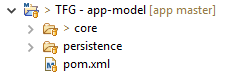
\includegraphics[
   keepaspectratio=true
]{./06_Implementacion/img/estructuramodeljava.png}
\caption{Estructura modulo model}
\end{figure}

En el submódulo \textit{persistence} se implementa toda la persistencia de datos, desde las clases persistentes hasta las definiciones e implementaciones de los \textit{DAOs}. Por su parte, en el submódulo \textit{core} se define e implementa la lógica de negocio.

Con esta separación en módulos conseguimos hacer más independiente cada uno de los módulos que formarán el desplegable de la aplicación. De tal manera, que si queremos utilizar otra implementación de persistencia, simplemente tenemos que reemplazar el \textit{JAR} generado por dicho módulo por el que queramos utilizar, en el archivo de aplicación web (WAR).

\subsubsection*{Estructura directorios Model - Persistence}
\begin{figure}[H]
\centering
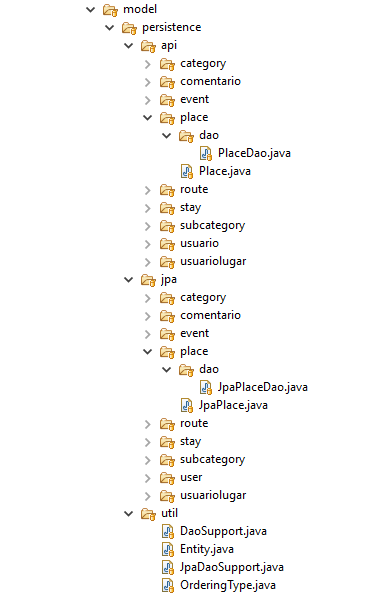
\includegraphics[
   keepaspectratio=true
]{./06_Implementacion/img/estructuramodelpersistence.png}
\caption{Estructura modulo model}
\end{figure}

\begin{itemize}
	\item \textbf{Directorio: ../model/persistence/api. } Es el directorio donde se encuentran todas las definiciones de las clases persistentes (Ej: Place.java) y los \textit{DAOs} (Ej: PlaceDao.java).
	\item \textbf{Directorio: ../model/persistence/jpa. } Directorio donde residen las implementaciones de las definiciones anteriores (Ej: JpaPlace.java, JpaPlaceDao.java). Como su nombre indica, se hace uso del API de persistencia JPA. 
	\item \textbf{Directorio: ../model/persistence/util. } Es el directorio donde se incluyen clases de utilidad (Ej: DaoSupport y JpaDapSupport, para la implementación de los \textit{DAOs}).
\end{itemize}

\subsubsection*{Estructura directorios Model - Core}
\begin{figure}[H]
\centering
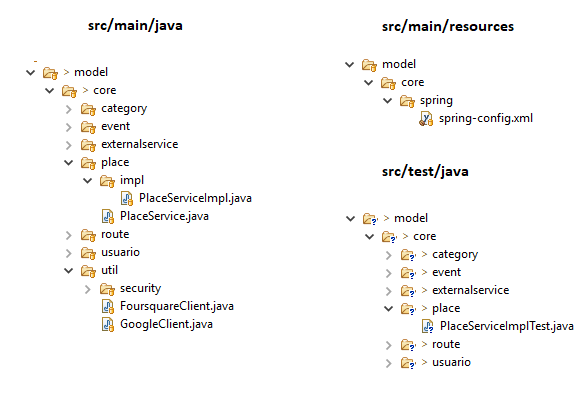
\includegraphics[
   keepaspectratio=true
]{./06_Implementacion/img/estructuramodelcore.png}
\caption{Estructura modulo model}
\end{figure}

\subsection{Estructura proyecto Ionic}


\section{Implementación del modelo}


\subsection{Persistencia}


\subsection{Consultas a la Base de datos}


\section{Implementación servicio REST}


\section{Implementación cliente web}


\subsection{Modelo}


\subsection{Controlador}


\subsection{Vista}


\section{Implementación cliente móvil}


\subsection{Modelo}


\subsection{Controlador}


\subsection{Vista}